9.3.a. Modify heat\_CN.m to solve the heat equation for $-1\leq x\leq1$ with step function initial data

$$u(x,0)=\left \{ \begin{array}{cc} 1 & x < 0 \\ 0 & x\geq 0 \end{array} \right.$$

With appropriate Dirichlet boundary conditions, the exact solution is

$$u(x,t)=\frac12\text{erfc}(x/\sqrt{4\kappa t})$$

where erfc is the complementary error function

$$\text{erfc}=\frac{2}{\sqrt{\pi}}\int_x^{\infty}e^{-z^2}dz.$$

i. Test this routine $m=39$ and $k=4h$. Note that there is an initial rapid transient decay of the high
wave numbers that is not captured well with this size time step.\\
ii. How small do you need to take the time step to get reasonable results? For a suitably small time
step, explain why you get much better results by using $m=38$ than $m=39$. What is the observed order of
accuracy as $k\rightarrow 0$ when $k=\alpha h$ with $\alpha$ suitably small and $m$ even?\\
b. Modify heat\_trbdf2.m (see Exercise 9.2) to solve the heat equation for $-1\leq x\leq1$ with step
function initial data as above. Test this routine using $k=4h$ and estimate the order of accuracy as
$k\rightarrow0$ with $m$ even. Why does the TR-BDF2 method work better than Crank-Nicolson?\\

\begin{solution}\renewcommand{\qedsymbol}{}\ \\
    a.i.
    \begin{center}
        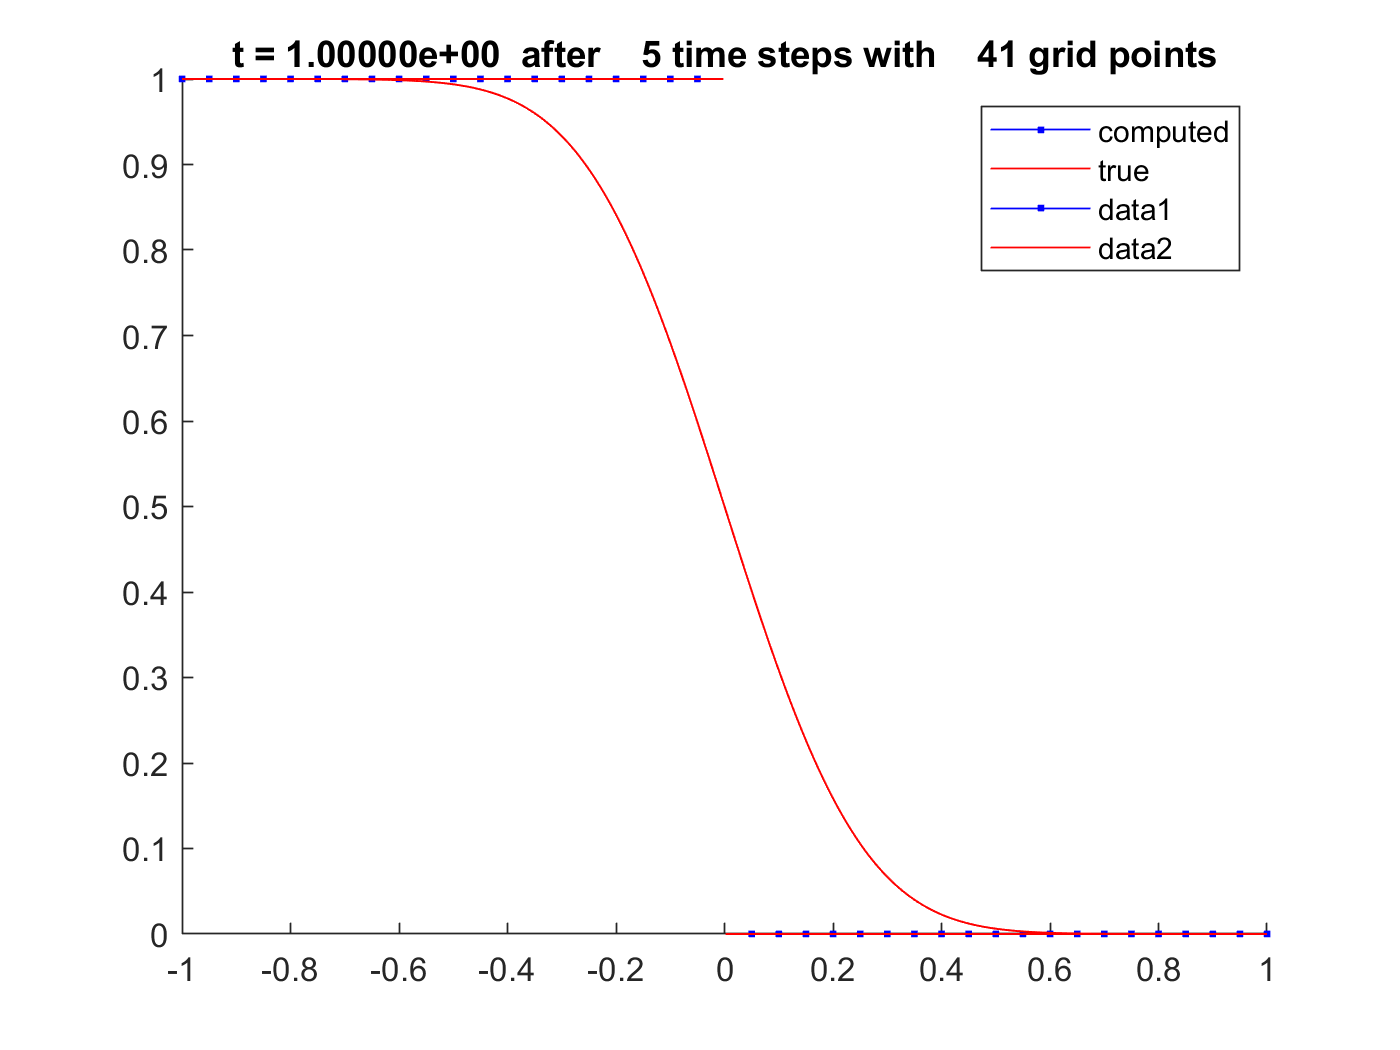
\includegraphics[scale=0.3]{3a.PNG}
    \end{center}
        
    ii. Here we are taking a time step of $k=\frac{1}{10}h$.
    \begin{center}
        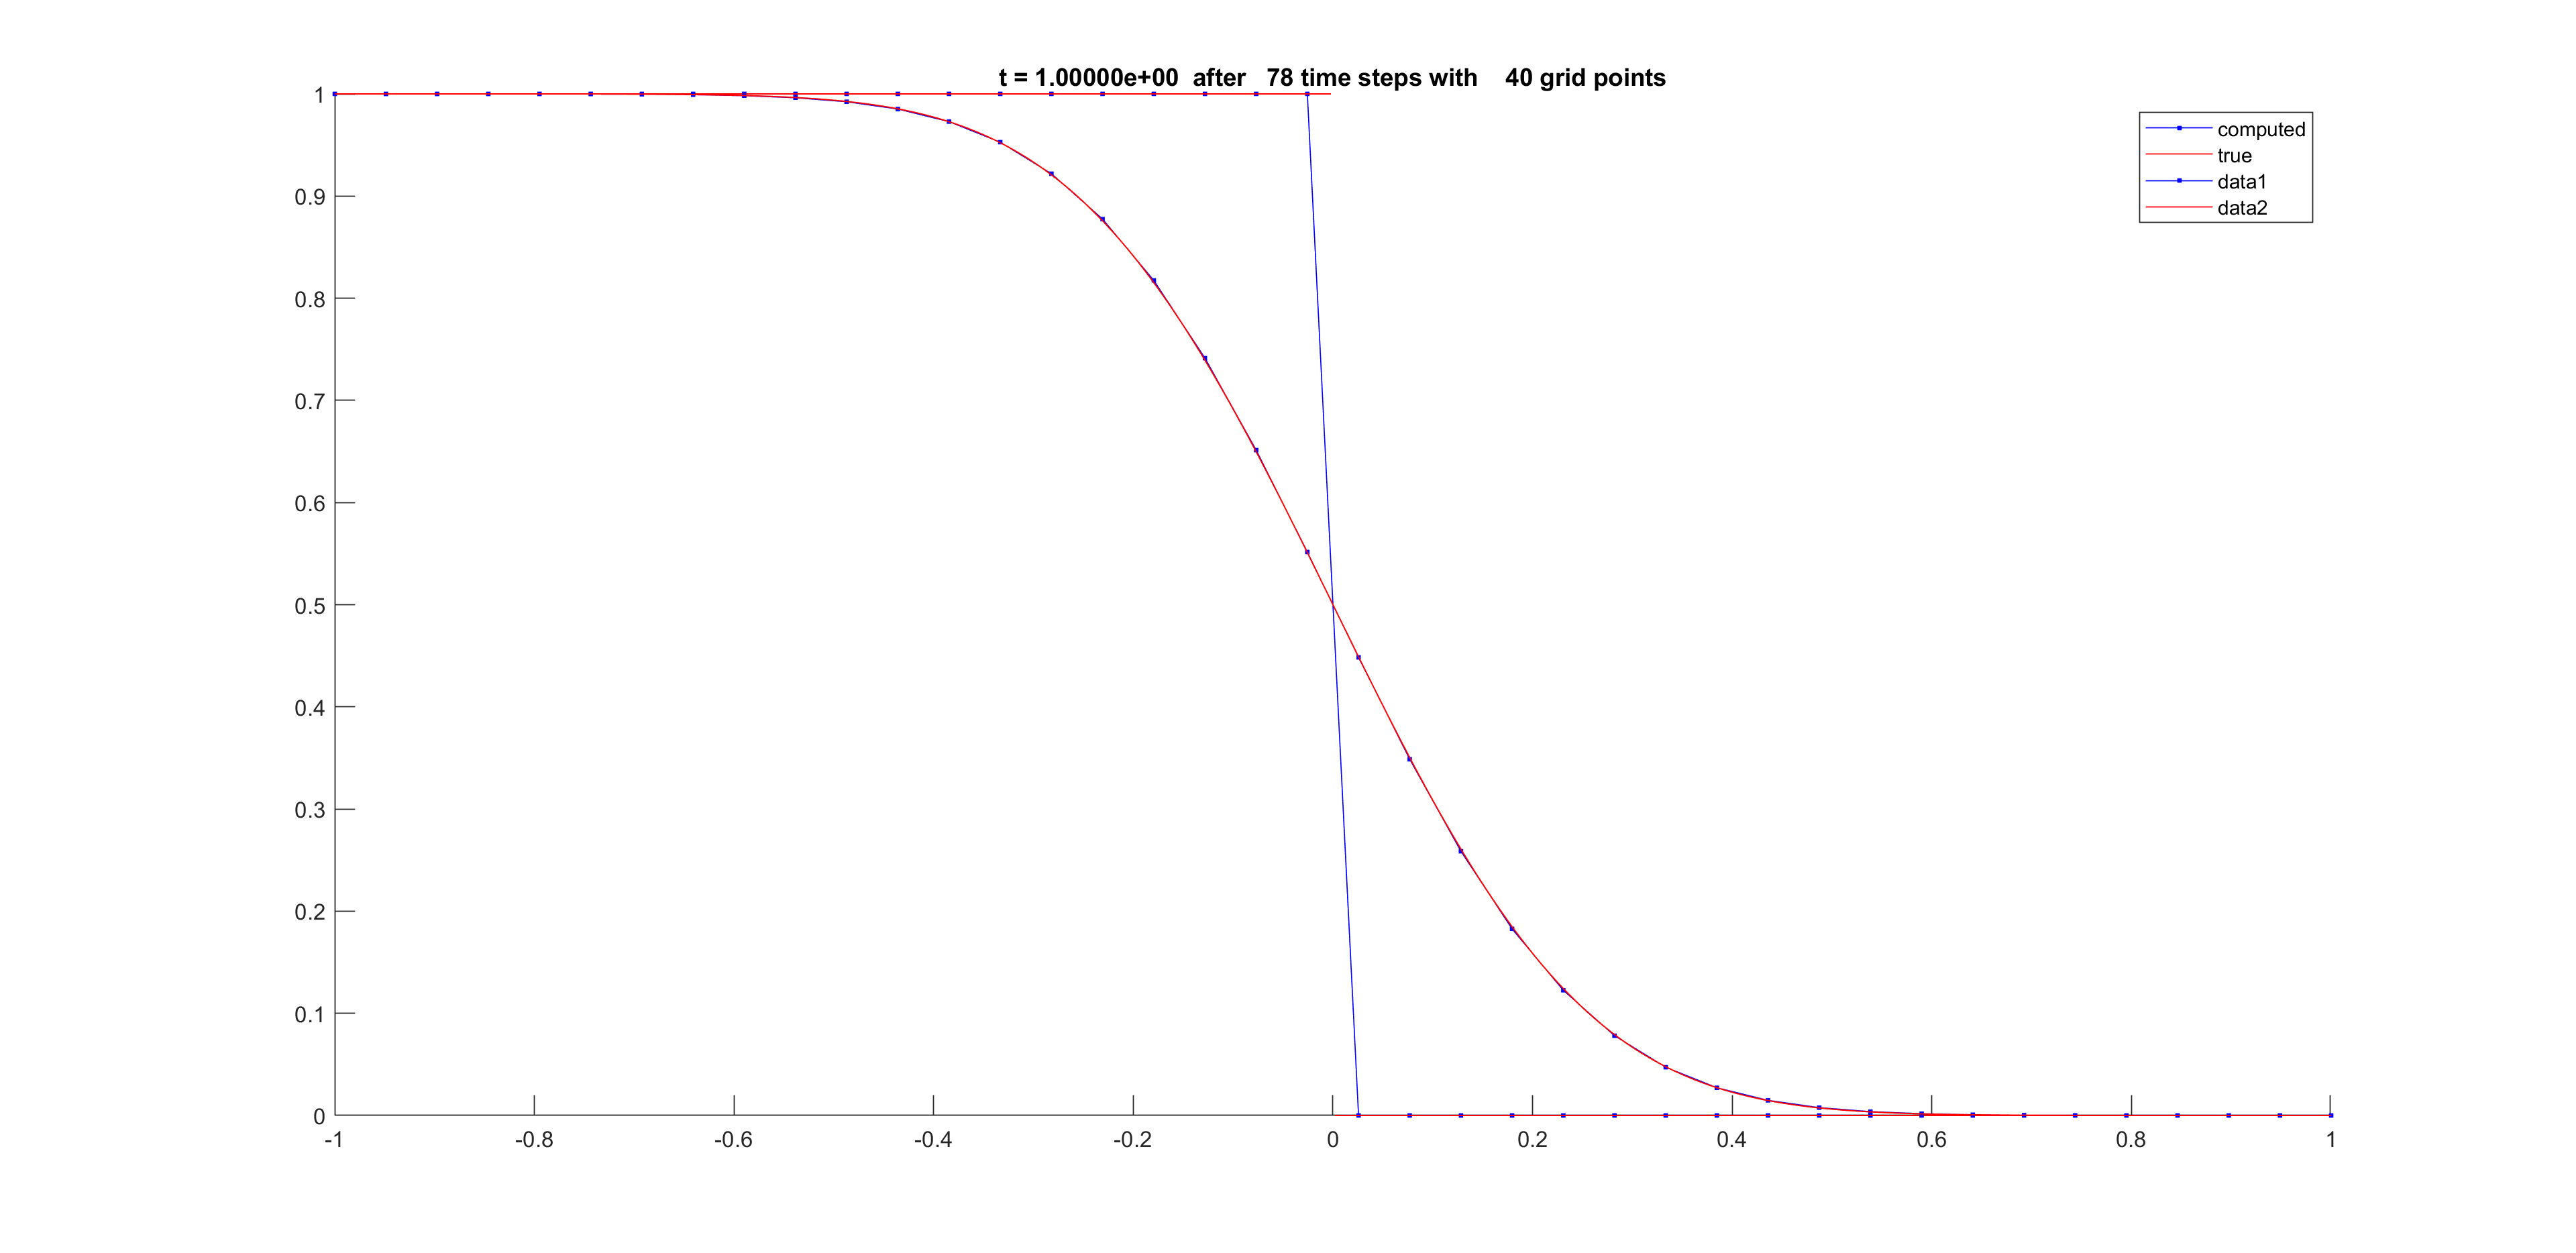
\includegraphics[scale=0.15]{3a2.PNG}
    \end{center}
        
    b. The TR-BDF2 works better than the Crank-Nicolson due to the better performance with the same time
    step.
    \begin{center}
        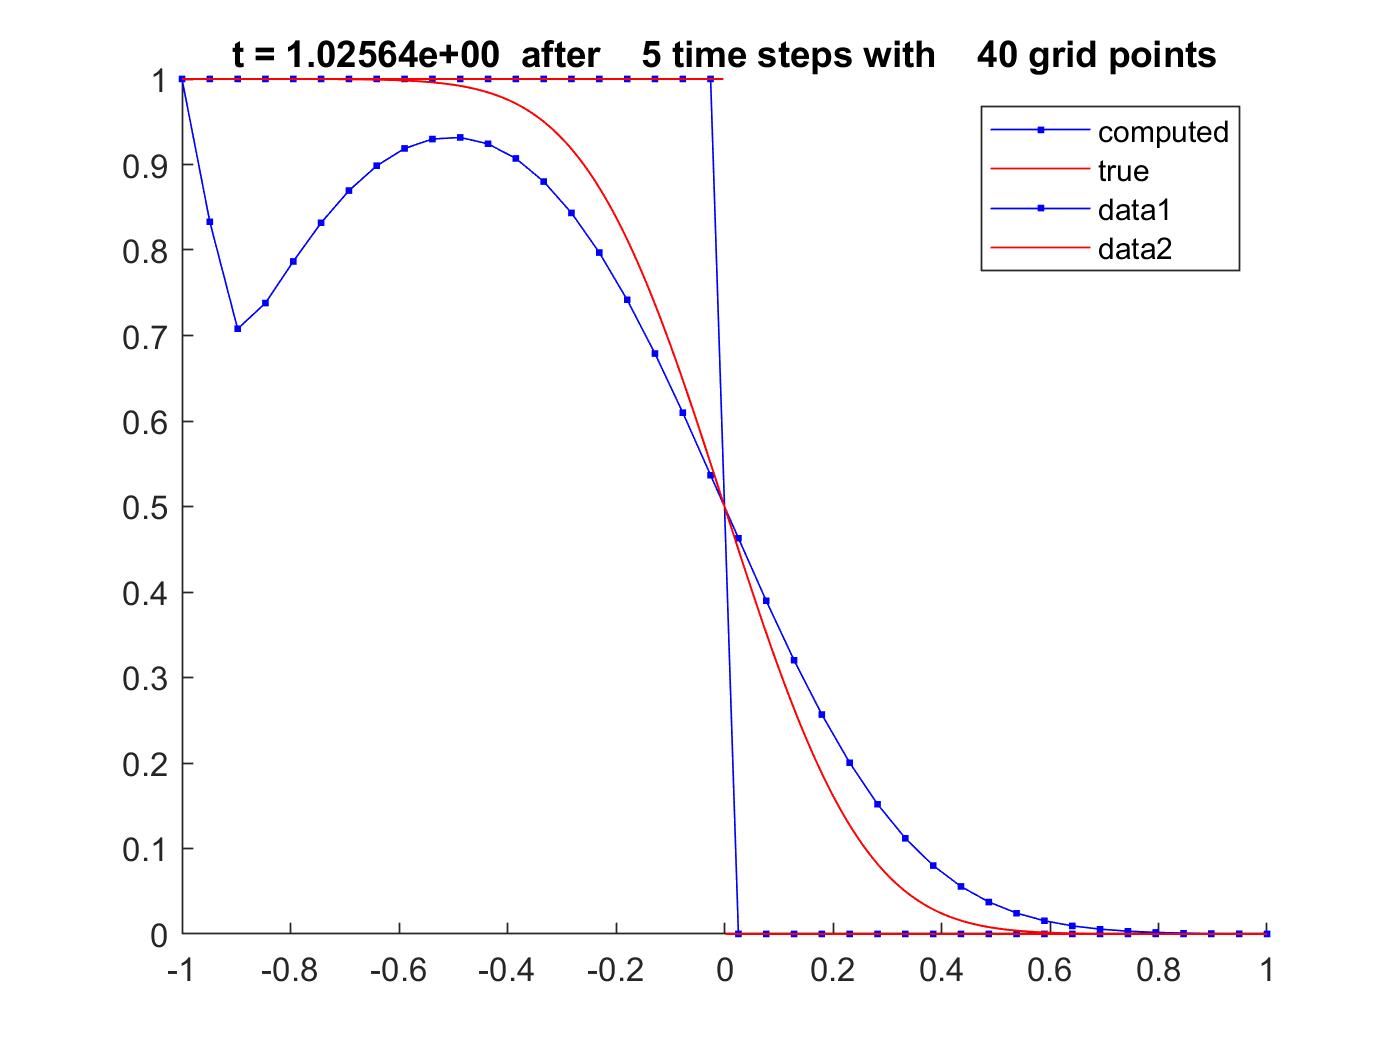
\includegraphics[scale=0.3]{3b.PNG}
    \end{center}

\end{solution}

\newpage
\lstinputlisting{heat_CNstep.m}
\newpage
\lstinputlisting{heat_trbdf2step.m}